\chapter{Symétries axiale et centrale}

\activites

\begin{activite}[Miroir, mon beau miroir]
\begin{center} 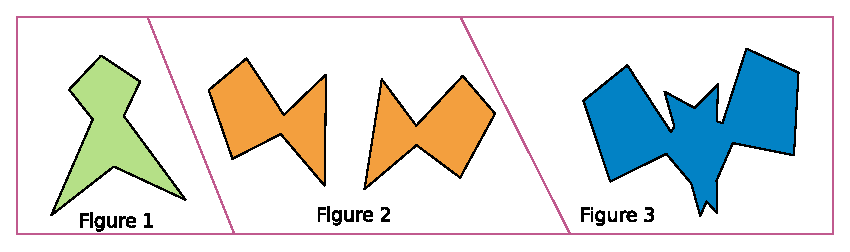
\includegraphics[width=14.5cm]{miroir} \end{center}

\begin{partie}
Observe les trois figures ci‑dessus :
\begin{enumerate}
 \item Quel est leur point commun ?
 
Comment peux‑tu le mettre en évidence ?
 \item Dans des publicités ou des magazines, trouve des images ou des logos qui ont la même propriété.
 \end{enumerate}
\end{partie}

\begin{minipage}[c]{0.54\linewidth}
\begin{partie}
À l'aide de papier calque, complète la figure ci‑contre avec un minimum de tracés pour que la droite d soit son \textbf{axe de symétrie}.
\end{partie}
\end{minipage}
\begin{minipage}[c]{0.44\linewidth}
\begin{center} 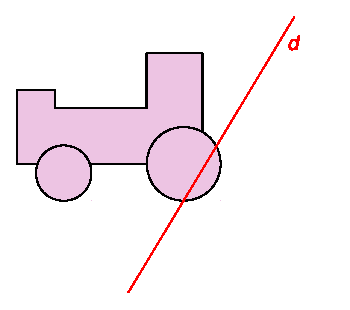
\includegraphics[width=4.5cm]{train} \end{center}
\end{minipage} \\

\end{activite}

%%%%%%%%%%%%%%%%%%%%%%%%%%%%%%%%%%%%%%%%%%%%%%%%%%%%%%%%%%%%%%%%%

\begin{activite}[Le symétrique dans l'œil]

\begin{center}
\begin{tabularx}{1.05\linewidth}{XXXX}
\begin{center} 
\includegraphics[width=3cm]{oeil1} \end{center} & \begin{center} 
\includegraphics[width=2.5cm]{oeil2} \end{center} & \begin{center} 
\includegraphics[width=3.2cm]{oeil3} \end{center} & \begin{center} 
\includegraphics[width=3.5cm]{oeil4} \end{center} \\
\begin{center} Figure 1 \end{center} & \begin{center} Figure 2 \end{center} & \begin{center} Figure 3 \end{center} & \begin{center} Figure 4 \end{center} \\
 \end{tabularx}
 \end{center}

\begin{partie} \label{SymAxCent_acti}
Observe les figures ci-dessus. La figure bleue est‑elle toujours symétrique à la figure orange par rapport à la droite tracée ? Justifie ta réponse en écrivant une phrase.
\end{partie}

\begin{partie}
Reproduis les figures ci‑dessous. Complète‑les à main levée en respectant la symétrie par rapport à la droite d et en tenant compte des remarques faites dans la partie \ref{SymAxCent_acti}.

\begin{minipage}[c]{0.48\linewidth}
\begin{center} 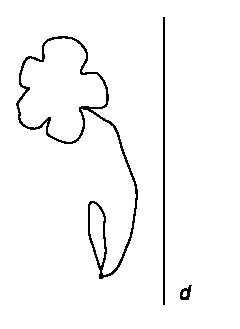
\includegraphics[width=3.5cm]{figure1} \end{center} 
 \end{minipage}
 \begin{minipage}[c]{0.48\linewidth}
 \begin{center} 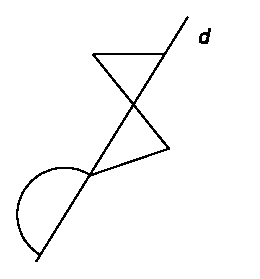
\includegraphics[width=3.5cm]{figure2} \end{center} 
  \end{minipage} \\
\end{partie}

\end{activite}

%%%%%%%%%%%%%%%%%%%%%%%%%%%%%%%%%%%%%%%%%%%%%%%%%%%%%%%%%%%%%%%%%

\begin{activite}[Une droite bien connue]

\begin{minipage}[c]{0.64\linewidth}
\begin{partie}
Sur la figure ci‑contre, quel est le symétrique du point $A$ par rapport à l'axe $d$ ? \\[0.5em]
Trouve les paires de points symétriques par rapport à la droite $d$. Décalque‑les ainsi que la droite $d$.
\end{partie}

\begin{partie}
Quel est le symétrique du point $J$ par rapport à l'axe $d$ ? Y a‑t‑il un autre point qui a la même particularité ?
\end{partie}

\begin{partie}
Sur ton calque, relie les points qui sont symétriques. Que peux-tu dire de la droite $d$ pour ces segments ?
\end{partie}
 \end{minipage}
  \qquad \begin{minipage}[c]{0.30\linewidth}
  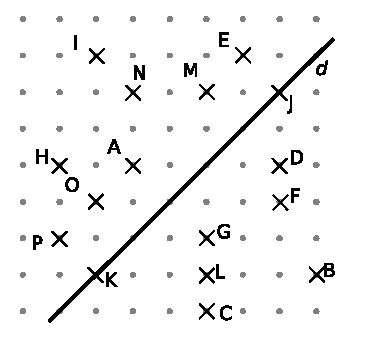
\includegraphics[width=5.5cm]{droite_connue}
  \end{minipage} \\
 

\begin{partie}
Trace le cercle de centre $J$ passant par $A$ et celui de centre $K$ passant par $A$. Que remarques‑tu ?
         
Trace un autre cercle passant par $A$ et $G$. Où doit se situer son centre ?
\end{partie}


\begin{partie}
Sur ton calque, place un point $T$ qui n'est pas sur la droite $d$. Propose deux façons de construire son symétrique $T'$ par rapport à $d$ sans plier le calque.
\end{partie}

\end{activite}

%%%%%%%%%%%%%%%%%%%%%%%%%%%%%%%%%%%%%%%%%%%%%%%%%%%%%%%%%%%%%%%%%

\begin{activite}[Un peu de mesure]

\begin{partie}[Symétrique d'un segment]
\begin{enumerate}
 \item Trace une droite $d$ et un segment $[AB]$. Construis le symétrique du segment $[AB]$ par rapport à la droite $d$.
 \item Compare les mesures des deux segments. Tes camarades obtiennent‑ils la même remarque ?
 
 \begin{minipage}[c]{0.52\linewidth}
 \item Romain avait construit le symétrique $A'B'C'$ du triangle $ABC$ par rapport à l'axe $d$. Malheureusement, sa feuille s'est déchirée et il ne reste que la figure ci‑contre. Romain doit déterminer le périmètre du triangle $ABC$. 
 
Explique comment il peut faire en utilisant uniquement la règle graduée et sans tracé supplémentaire.
  \end{minipage}
   \qquad \begin{minipage}[c]{0.46\linewidth}
  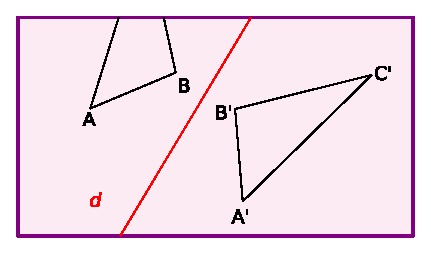
\includegraphics[width=5.5cm]{feuille_Romain}
  \end{minipage} \\
 \end{enumerate}
\end{partie}

\begin{partie}[Symétrique d'un cercle]
\begin{enumerate}
 \begin{minipage}[c]{0.62\linewidth}
 \item Reproduis la figure ci‑contre, place un point $M$ sur le cercle (\phantom{...}) puis construis les points $O'$ et $M'$ symétriques respectifs de $O$ et de $M$ par rapport à $d$.
 
Quelle est la longueur de $[O'M']$ ? Justifie ta réponse.
 \item Construis le symétrique du cercle (\phantom{...}) par rapport à la droite $d$.
  \end{minipage}
   \qquad \begin{minipage}[c]{0.36\linewidth}
  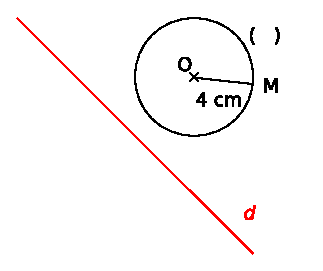
\includegraphics[width=4.5cm]{cercle_sym}
  \end{minipage} \\
 \end{enumerate}
\end{partie}

\end{activite}

%%%%%%%%%%%%%%%%%%%%%%%%%%%%%%%%%%%%%%%%%%%%%%%%%%%%%%%%%%%%%%%%%

\begin{activite}[Symétrique d'une droite]

\begin{minipage}[c]{0.62\linewidth}
\begin{partie}[Droite parallèle à l'axe]
\begin{enumerate}
 \item Trace deux droites parallèles \textcolor{B2}{$d$} et $d_1$ ;
 \item Construis la droite $d_2$ symétrique de la droite $d_1$ par rapport à l'axe \textcolor{B2}{$d$} ;
 \item Que peux‑tu dire des droites $d_1$ et $d_2$ ? Justifie ta réponse.
 \end{enumerate}
\end{partie}
 \end{minipage}
   \qquad \begin{minipage}[c]{0.36\linewidth}
  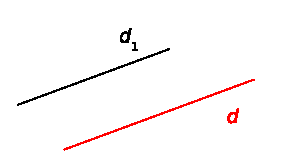
\includegraphics[width=4.5cm]{d1d}
  \end{minipage} \\

\vspace{1em}

\begin{minipage}[c]{0.62\linewidth}
\begin{partie}[Droite perpendiculaire à l'axe]
\begin{enumerate}
 \item Construis deux droites \textcolor{B2}{$d$} et $d_1$ perpendiculaires ;
 \item Place un point $A$ sur la droite $d_1$ et construis son symétrique $A'$ par rapport à l'axe \textcolor{B2}{$d$}. Justifie la position du point $A'$. \\[0.5em]
Que peux-tu dire alors de la droite $d_2$ symétrique de la droite $d_1$ par rapport à l'axe $d$ ?
 \end{enumerate}
\end{partie}
 \end{minipage}
   \qquad \begin{minipage}[c]{0.36\linewidth}
  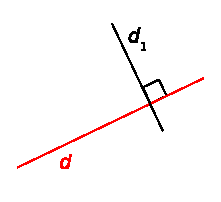
\includegraphics[width=3.5cm]{d1_perp_d}
  \end{minipage} \\

\end{activite}

%%%%%%%%%%%%%%%%%%%%%%%%%%%%%%%%%%%%%%%%%%%%%%%%%%%%%%%%%%%%%%%%%

\begin{activite}[Calque et demi-tour]

Mathieu a décalqué le bateau rose puis il l'a fait tourner autour du point $O$ dans le sens de la flèche. Il a dessiné quatre bateaux de couleurs différentes.

\vspace{1em}

\begin{minipage}[c]{0.42\linewidth}
\begin{partie}
Certains bateaux sont à moins d'un demi-tour, d'autres à plus d'un demi-tour du bateau de départ. Peux-tu préciser lesquels ?
\end{partie}

\begin{partie}
Reproduis, sur ton cahier, le bateau rose et le point $O$. À l'aide d'un morceau de papier calque, place un bateau qui soit à moins d'un demi-tour et un autre qui soit à plus d'un demi-tour du bateau de départ.
\end{partie}

\begin{partie} \label{SymAxCentActi2}
Mathieu remarque que lorsqu'il fait tourner le bateau rose autour du point $O$, le point $A$, tout en haut du mât, décrit une ligne qu'il connaît bien. Quelle est cette ligne ? Construis-la sur ton dessin.
\end{partie}
 \end{minipage}
   \quad \begin{minipage}[c]{0.36\linewidth}
  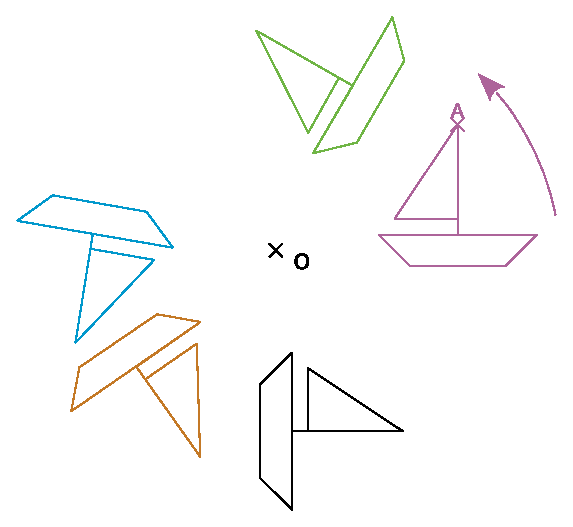
\includegraphics[width=8cm]{bateaux}
  \end{minipage} \\

\begin{partie} \label{SymAxCentActi3}
Mathieu aimerait bien construire un bateau qui soit exactement à un demi-tour du bateau rose. Pour savoir où s'arrêter de tourner, Mathieu se dit qu'il faudrait connaître la position exacte du point $A$ après un demi-tour. Construis ce point.
\begin{center} \textbf{\textcolor{H1}{Le demi-tour autour du point $O$ est encore appelé symétrie de centre $O$.}} \end{center}
\end{partie}

\begin{partie}
En t'aidant des parties \ref{SymAxCentActi2} et \ref{SymAxCentActi3}, construis le symétrique du bateau de départ par la symétrie de centre $O$.
\end{partie}

\end{activite}

%%%%%%%%%%%%%%%%%%%%%%%%%%%%%%%%%%%%%%%%%%%%%%%%%%%%%%%%%%%%%%%%%

\begin{activite}[Dans un quadrillage]

\begin{minipage}[c]{0.62\linewidth}
\begin{partie}
Reproduis la figure ci-contre sur ton cahier. \\[0.5em]
Pour aller de $O$ à $A$, on suit la flèche rose puis la verte.
\end{partie}
 \end{minipage}
  \qquad \begin{minipage}[c]{0.36\linewidth}
  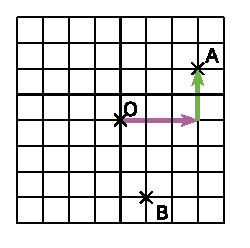
\includegraphics[width=3.7cm]{quadrillageAOB}
  \end{minipage} \\

\begin{partie}
En utilisant du papier calque, construis le symétrique de chaque flèche par rapport à $O$ puis complète les phrases suivantes : 
\begin{itemize}
 \item Le symétrique par rapport à un point d'une flèche de trois carreaux vers la droite est une flèche \ldots ;
 \item Le symétrique par rapport à un point d'une flèche de deux carreaux vers le haut est \ldots.
 \end{itemize}
\end{partie}
                
\begin{partie}
À l'aide des symétriques des flèches rose et verte, place le point $A'$, symétrique du point $A$ par rapport à $O$.
\end{partie}
         
\begin{partie}
En utilisant uniquement le quadrillage et en t'inspirant de la méthode découverte ci-dessus, place le point $B'$ symétrique du point $B$ par rapport à $O$.
\end{partie}

\end{activite}

%%%%%%%%%%%%%%%%%%%%%%%%%%%%%%%%%%%%%%%%%%%%%%%%%%%%%%%%%%%%%%%%%

\begin{activite}[Centre de symétrie]

\begin{partie}
Construis un segment $[RS]$ de 5 cm de longueur. Quel est son centre de symétrie ?
\end{partie}


\begin{partie}
Construis un cercle de centre $O$ et de rayon 3 cm. Quel est son centre de symétrie ?
\end{partie}
         
         
\begin{partie}
Construis une droite $d$. Combien admet-elle de centres de symétrie ?
\end{partie}
         
         
\begin{partie}
Est-il possible de construire un triangle non aplati qui a un centre de symétrie ?
\end{partie}
         
         
\begin{partie}
Place trois points non alignés $A$, $B$ et $O$. Construis les points $C$ et $D$ pour que le quadrilatère $ABCD$ ait le point $O$ comme centre de symétrie.
\end{partie}
        
\vspace{1em}

\begin{minipage}[c]{0.62\linewidth}
\begin{partie}
Sur ton cahier, place trois points $Z$, $V$ et $W$ comme sur la figure ci-contre. Comment construire le point $M$ pour que le quadrilatère $ZVWM$ ait un centre de symétrie ?
\end{partie}         
              
         
\begin{partie}
Construis un hexagone $EFGHIJ$ qui admet un centre de symétrie.
\end{partie}
 \end{minipage}
  \qquad \begin{minipage}[c]{0.36\linewidth}
  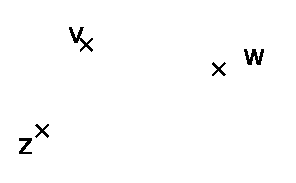
\includegraphics[width=4.5cm]{pointsVWZ}
  \end{minipage} \\

\end{activite}

%%%%%%%%%%%%%%%%%%%%%%%%%%%%%%%%%%%%%%%%%%%%%%%%%%%%%%%%%%%%%%%%%

\cours
%\section{Une section}

% remarque : pour qu'un mot se retrouve dans le lexique : \MotDefinition{asymptote horizontale}{} 

\begin{methode*1}[Construire le symétrique d'un point à l'équerre]

\begin{aconnaitre}
Le \MotDefinition{symétrique d'un point $P$}{} par rapport à une droite $d$ est le point $S$ tel que la droite $d$ soit la médiatrice du segment $[PS]$. 
\end{aconnaitre}

\begin{exemple*1}
Construis le point $S$, symétrique de $P$ par rapport à la droite $d$, en utilisant l'équerre : \\[0.5em]
\begin{tabularx}{\textwidth}{X|X|X}
 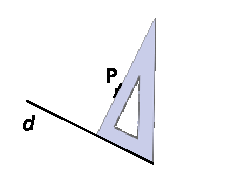
\includegraphics[width=2.4cm]{equerredP} &  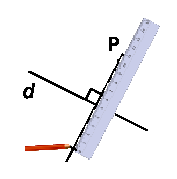
\includegraphics[width=2.4cm]{equerredP_perp} & \includegraphics[width=2.2cm]{symP} \\ 
 On construit la droite perpendiculaire à la droite $d$ passant par le point $P$. & On reporte la distance de $P$ à $(d)$ de l'autre côté de $d$ sur cette perpendiculaire. & On obtient ainsi le point $S$ tel que $d$ soit la médiatrice de $[PS]$.\\
\end{tabularx} \\
 \end{exemple*1}


\exercice
Trace deux droites sécantes $d'$ et $d''$ puis place un point $A$ qui n'appartient ni à $d'$, ni à $d''$. Construis les symétriques $A'$ et $A''$ de $A$ par rapport à $d'$ et à $d''$.
%\correction
 
\end{methode*1}

%%%%%%%%%%%%%%%%%%%%%%%%%%%%%%%%%%%%%%%%%%%%%%%%%%%%%%%%%%%%%%%%%%%%%

\begin{methode*1}[Construire le symétrique d'un point au compas]

\begin{aconnaitre}
Si $A$ et $B$ sont symétriques par rapport à une droite $d$ alors chaque point de la droite $d$ est \MotDefinition{équidistant}{} de $A$ et de $B$. 
\end{aconnaitre}

\begin{exemple*1}
Construis le point $S$, symétrique de $P$ par rapport à la droite $d$, au compas seul : \\[0.5em]
\begin{tabularx}{\textwidth}{X|X|X}
 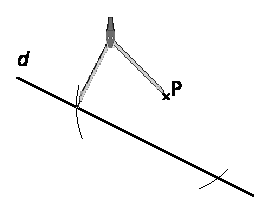
\includegraphics[width=3cm]{compasdP} &  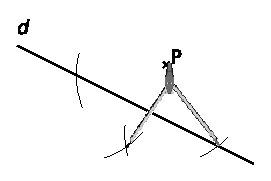
\includegraphics[width=3cm]{compasdP2} & 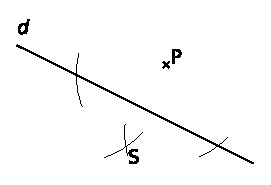
\includegraphics[width=3cm]{pointsdPS} \\ 
 On trace un arc de cercle de centre $P$ qui coupe l'axe en deux points. & De l'autre côté de la droite $d$, on trace deux arcs de cercle de même rayon et de centre les deux points précédents. & Ces deux arcs se coupent en un point qui est le point $S$, symétrique de $P$ par rapport à $d$. \\
\end{tabularx} \\
 \end{exemple*1}


\exercice
Construis un triangle $ABC$. Construis le point $D$, symétrique de $B$ par rapport à $(AC)$.
%\correction
 
\end{methode*1}

%%%%%%%%%%%%%%%%%%%%%%%%%%%%%%%%%%%%%%%%%%%%%%%%%%%%%%%%%%%%%%%%%%%%%

\begin{methode*1}[Utiliser les propriétés de la symétrie axiale]

\begin{aconnaitre}
La symétrie axiale conserve les \textbf{longueurs, l'alignement, les angles et les aires}.
\end{aconnaitre}

\begin{exemple*1}
Soit un triangle $ABC$ rectangle en $B$ tel que $AB = 3,3$ cm et $BC = 6$ cm. Quelle est la nature du triangle $A'B'C'$ symétrique de $ABC$ par rapport à la droite $(AC)$ ? Justifie. \\[0.5em]
\begin{minipage}[c]{0.4\linewidth}
 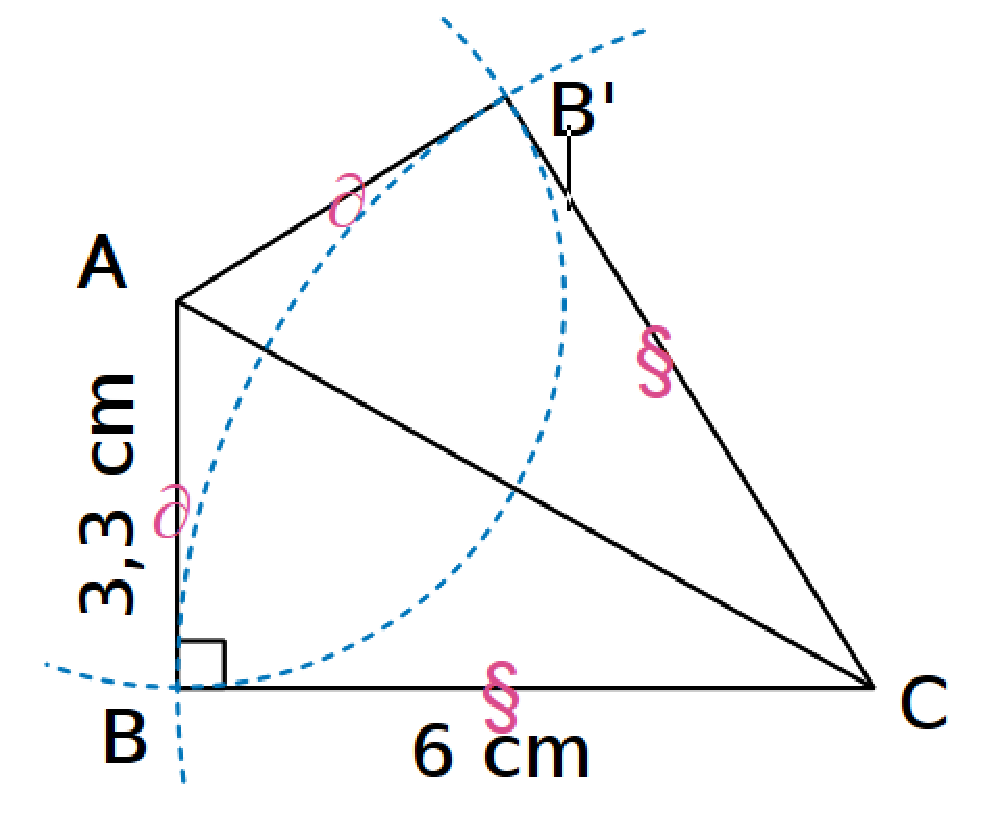
\includegraphics[width=4.3cm]{symABBC} \qquad
 \end{minipage}
 \begin{minipage}[c]{0.56\linewidth}
 \begin{itemize}
  \item $A$ et $C$ appartiennent à l'axe de symétrie, ils sont donc chacun leur propre symétrique. On appelle $B'$ le symétrique de $B$ par rapport à $(AC)$.
  \item $ABC$ est rectangle en $B$ donc $\widehat{ABC} = 90^{\circ}$. Or la symétrie axiale conserve la mesure des angles donc $\widehat{A'B'C'} = 90^{\circ}$. $A'B'C'$ est un triangle rectangle en $B'$.
  \item La symétrie axiale conserve les longueurs donc $AB = AB' = 3,3$ cm et $CB = CB' = 6$ cm.
  \end{itemize}
 \end{minipage} \\
 \end{exemple*1}


\exercice
Trace une droite $d$ et un point $F$ qui n'est pas sur $d$. Trace le cercle de centre $F$ et de rayon 5 cm. Trace son symétrique par rapport à $d$.
%\correction
 
\end{methode*1}

%%%%%%%%%%%%%%%%%%%%%%%%%%%%%%%%%%%%%%%%%%%%%%%%%%%%%%%%%%%%%%%%%%%%%

\begin{methode*1}[Construire le symétrique d'un point]

\begin{aconnaitre}
\MotDefinition{Deux points $A$ et $A'$ sont symétriques par rapport à $O$}{} lorsque $O$ est le milieu du segment $[AA']$. 
\end{aconnaitre}

\begin{exemple*1}
Trace le point $A'$ tel que les points $A$ et $A'$ soient symétriques par rapport à $O$ : \\[0.5em]
\begin{tabularx}{\textwidth}{X|X|X}
 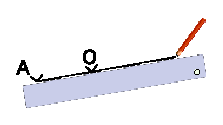
\includegraphics[width=3cm]{regleAO} &  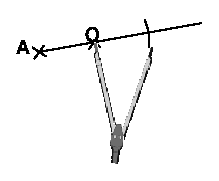
\includegraphics[width=3cm]{compasAO} & 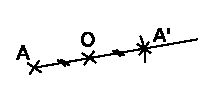
\includegraphics[width=3cm]{pointsAOA} \\ 
 On trace la demi-droite $[AO)$. & On trace un arc de cercle de centre $O$ et de rayon $OA$. Il coupe la demi-droite $[AO)$ en un point. & On place le point $A'$ à l'intersection de la demi-droite $[AO)$ et de l'arc de cercle. On code la figure. \\
\end{tabularx} \\
 \end{exemple*1}


\exercice
Trace un segment $[AB]$ de 5 cm de longueur puis construis le point $C$ symétrique de $B$ par rapport à $A$.
%\correction

\exercice
Trace un segment $[RT]$ de 8,4 cm de longueur, puis place le point $W$ tel que $R$ et $T$ soient symétriques par rapport au point $W$.
%\correction
 
\end{methode*1}

%%%%%%%%%%%%%%%%%%%%%%%%%%%%%%%%%%%%%%%%%%%%%%%%%%%%%%%%%%%%%%%%%%%%%

\begin{methode*1}[onstruire le symétrique d'une figure]

\begin{aconnaitre}
\MotDefinition{Deux figures symétriques par rapport à un point}{} sont superposables après un demi-tour autour de ce point. 
\end{aconnaitre}

\begin{exemple*1}
Construis le symétrique de la figure $ABCD$ par rapport au point $O$ : \\[0.5em]
\begin{tabularx}{\textwidth}{X|X|X}
 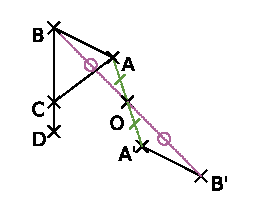
\includegraphics[width=3cm]{figure_sym1} &  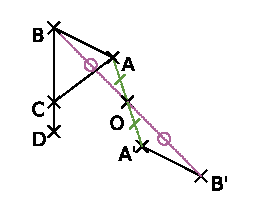
\includegraphics[width=3cm]{figure_sym2} & 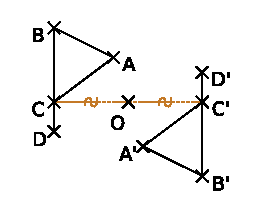
\includegraphics[width=3cm]{figure_sym3} \\ 
 On construit les points $A'$ et $B'$, symétriques des points $A$ et $B$ par rapport à $O$. On trace le segment $[A'B']$. & On construit  le point $D'$, symétrique du point $D$ par rapport à $O$. On trace le segment $[B'D']$. & On construit le point $C'$, symétrique du point $C$ par rapport à $O$. On trace le segment $[A'C']$. \\
\end{tabularx} \\
 \end{exemple*1}


\exercice
Trace un rectangle $ABCD$ tel que $AB = 4$ cm et $BC = 2,5$ cm. Trace le cercle de centre $B$ passant par $C$. Construis le symétrique de cette figure par rapport au point $D$.
%\correction
 
\end{methode*1}

%%%%%%%%%%%%%%%%%%%%%%%%%%%%%%%%%%%%%%%%%%%%%%%%%%%%%%%%%%%%%%%%%%%%%

\begin{methode*1}[Utiliser les propriétés de la symétrie centrale]

\begin{aconnaitre}
Si deux segments sont symétriques par rapport à un point alors \textbf{ils ont la même longueur}.

Si deux angles sont symétriques par rapport à un point alors \textbf{ils ont la même mesure}.

La symétrie centrale \textbf{conserve le périmètre et l'aire}.
\end{aconnaitre}

\begin{exemple*1}
Un triangle $PIC$ a un périmètre de 16,4 cm. Quel est le périmètre du triangle $PI'C'$ image de $PIC$ par la symétrie de centre $P$ ? Justifie ta réponse.\\[1em]
\correction
Les triangles $PIC$ et $PI'C'$ sont symétriques par rapport à un point : ils ont donc le même périmètre, c'est à dire 16,4 cm.
 \end{exemple*1}


\exercice
Les angles $\widehat{xOy}$ et $\widehat{x'Oy'}$, dont les mesures respectives sont $54^{\circ}$ et $55^{\circ}$, sont-ils symétriques par rapport au point $O$ ? Justifie ta réponse.
%\correction

\exercice
$ESV$ est un triangle rectangle en $E$. Quelle est la nature du triangle $E'S'V'$ image de $ESV$ par une symétrie centrale ? Justifie ta réponse.
%\correction
 
\end{methode*1}



\exercicesbase
\begin{colonne*exercice}

\serie{Symétrie axiale}

\begin{exercice}[Figures symétriques ?]
Dans chaque cas, indique si les figures verte et orange sont symétriques par rapport à une droite.
\begin{center} 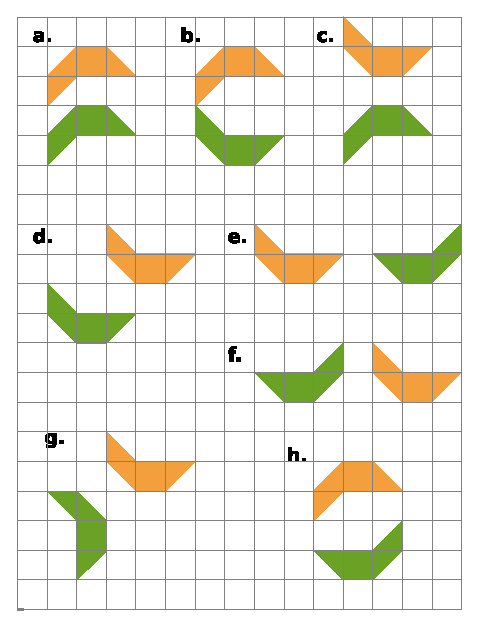
\includegraphics[width=7.9cm]{figures_sym} \end{center}
\end{exercice}


\begin{exercice}[Figures symétriques ? (bis)]
Dans chaque cas, indique si les figures mauve et bleue sont symétriques par rapport à une droite.
\begin{center} 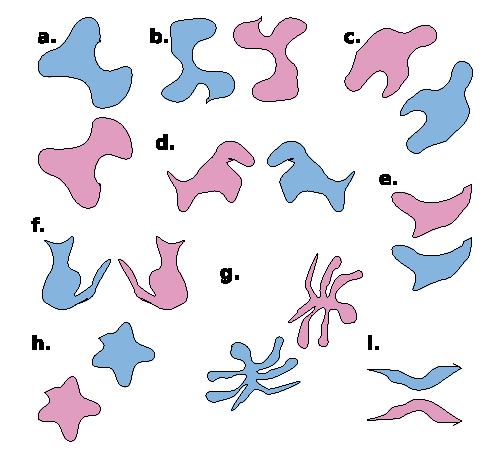
\includegraphics[width=8.1cm]{figures_sym2} \end{center}
\end{exercice}


\begin{exercice}[Erreurs à trouver]
Pourquoi les figures ocre et verte ne sont-elles pas symétriques par rapport à la droite $d$ ?
\begin{center} 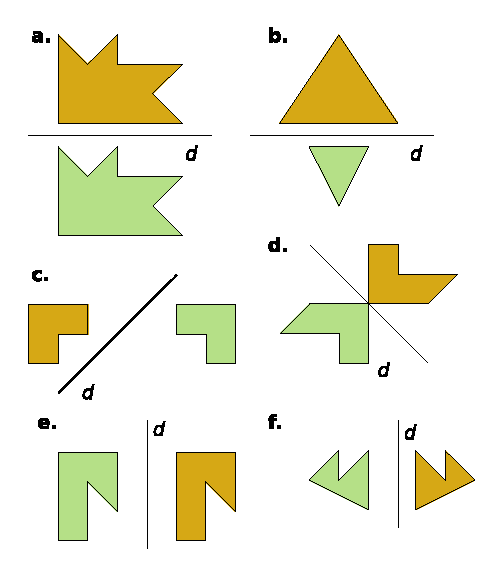
\includegraphics[width=7.9cm]{figures_erreurs} \end{center}
\end{exercice}


\begin{exercice}[Figure à plier]
\begin{minipage}[c]{0.62\linewidth}
Sur du papier calque, trace une droite rouge. Cette droite partage ton calque en deux.

Dessine un motif en t'inspirant du dessin ci‑contre sur la première moitié du calque, puis plie ton calque et complète ton dessin pour que ta figure soit symétrique par rapport à l'axe noir.
 \end{minipage} \hfill%
 \begin{minipage}[c]{0.36\linewidth}
 \begin{center} 
\includegraphics[width=1.7cm]{papillon} \end{center}
  \end{minipage} \\
\end{exercice}


\begin{exercice}[Jeu des différences]
Retrouve les erreurs qui se sont glissées sur ces deux figures pour qu'elles soient parfaitement symétriques par rapport à la droite rouge.
\begin{center} 
\includegraphics[width=5cm]{jeu_differences} \end{center}
\end{exercice}


\begin{exercice}[Points symétriques]
\begin{enumerate}
 \item Sur la figure ci‑dessous, cite les couples de points qui sont symétriques par rapport à l'axe rouge. \\[0.3em]
 \begin{center} 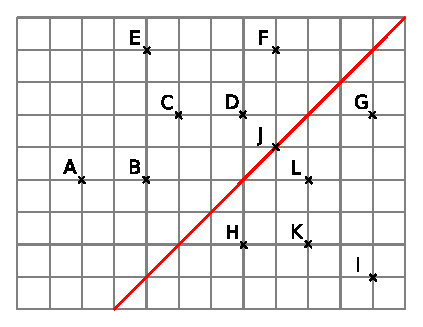
\includegraphics[width=6.9cm]{quadrillage_axerouge} \end{center}
 \item Fais trois phrases du type : « L'axe rouge est l'axe de symétrie du segment \ldots ».
 \item Reproduis cette figure et complète‑la pour que chaque point ait un symétrique.
 \end{enumerate}
\end{exercice}


\begin{exercice}[Cases croisées]
Reproduis et colorie le minimum de cases pour que l'axe rouge soit un axe de symétrie.
 \begin{center} 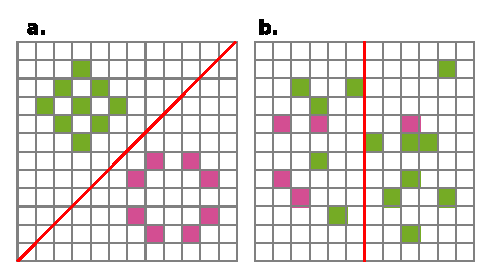
\includegraphics[width=8.1cm]{cases_croisees} \end{center}
\end{exercice}


\begin{exercice}[Frise]
Reproduis la figure ci‑dessous puis trace son symétrique par rapport à l'axe rouge. 
 \begin{center} 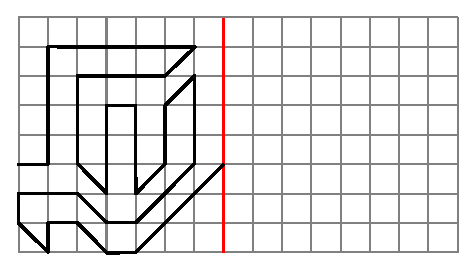
\includegraphics[width=7.9cm]{frise} \end{center}
\end{exercice}


\begin{exercice}
Reproduis puis trace le symétrique de chaque figure par rapport à $d$.

\begin{minipage}[c]{0.48\linewidth}
 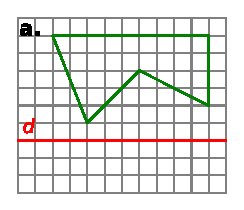
\includegraphics[width=3.7cm]{repro_d1}
 \end{minipage} \hfill%
 \begin{minipage}[c]{0.48\linewidth}
 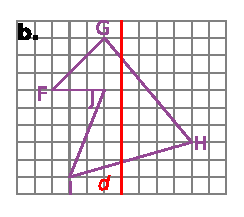
\includegraphics[width=3.7cm]{repro_d2}
  \end{minipage} \\
 \begin{minipage}[c]{0.48\linewidth}
 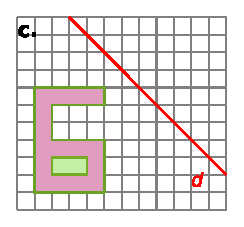
\includegraphics[width=3.7cm]{repro_d3}
 \end{minipage} \hfill%
 \begin{minipage}[c]{0.48\linewidth}
 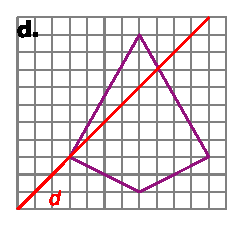
\includegraphics[width=3.7cm]{repro_d4}
 \end{minipage} \\
\end{exercice}


\begin{exercice}[Symétrique d'un point]
\begin{enumerate}
 \item Reproduis une figure similaire à celle ci‑dessous :
 \begin{center} 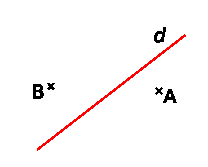
\includegraphics[width=2.8cm]{pointsABd} \end{center}
 \item Construis le symétrique par rapport à $d$ du point :
 \begin{itemize}
  \item $A$ à la règle et l'équerre ;
  \item $B$ au compas.
  \end{itemize}   
 \item Soit $H$ le point d'intersection de $(AB)$ avec $d$. Que dire de son symétrique par rapport à $d$ ?
 \end{enumerate} 
\end{exercice}


\begin{exercice}[Symétrique d'un triangle]
\begin{minipage}[c]{0.52\linewidth}
\begin{enumerate}
 \item Reproduis une figure similaire à celle ci-contre ;
 \item Construis au compas le symétrique du triangle $GHI$ par rapport à $d$.
 \end{enumerate}
 \end{minipage} \hfill%
 \begin{minipage}[c]{0.44\linewidth}
  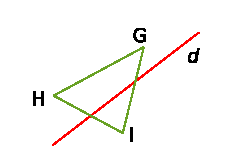
\includegraphics[width=3cm]{triangleGHId}
   \end{minipage} \\
\end{exercice}


\begin{exercice}[Symétrique d'un cercle]
\begin{enumerate}
 \item Trace un cercle $\mathcal{C}$ de centre $G$ et de rayon 5 cm. Place deux points $A$ et $B$ sur ce cercle non diamétralement opposés.
 \item Trace le symétrique de $\mathcal{C}$ par rapport à $(AB)$.
 \item Par quels points passent les deux cercles ? Justifie.
 \item Que se passe‑t‑il si $A$ et $B$ sont diamétralement opposés ?
 \end{enumerate}
\end{exercice}


\begin{exercice}[Symétrique d'une figure]
\begin{minipage}[c]{0.44\linewidth}
\begin{enumerate}
 \item Reproduis une figure similaire à celle ci‑contre ;
 \item À l'aide d'une règle et d'une équerre, trace le symétrique de cette figure par rapport à la droite $(AB)$.
 \end{enumerate}
 \end{minipage} \hfill%
 \begin{minipage}[c]{0.52\linewidth}
  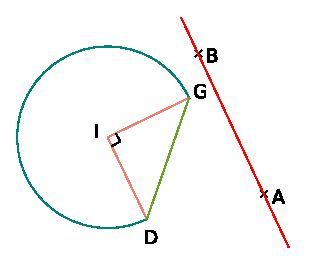
\includegraphics[width=4.5cm]{figure_droiteAB}
   \end{minipage} \\
\end{exercice}


\begin{exercice}[À propos des distances]
\begin{enumerate}
 \item Reproduis une figure similaire à celle ci‑dessous : 
 \begin{center} 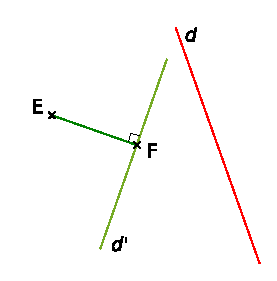
\includegraphics[width=4.7cm]{distances} \end{center}
 \item Trace le symétrique de $[EF]$ par rapport à $d$. On le note $[E'F']$. Que peux‑tu dire de la longueur de $[E'F']$ ? Justifie.
 \item Que peux‑tu dire du symétrique de $d'$ par rapport à $d$ ? Trace alors ce symétrique.
 \item Que peux‑tu dire du symétrique du cercle de diamètre $[EF]$ par rapport à $d$ ? Justifie.
 \end{enumerate}
\end{exercice}


\begin{exercice}[À propos de l'alignement]
\begin{enumerate}
 \item Trace une droite $d$. Place trois points $A$, $B$ et $C$ alignés qui n'appartiennent pas à $d$ ;
 \item Construis les points $A'$, $B'$ et $C'$ symétriques respectifs de $A$, $B$ et $C$ par rapport à $d$ ;
 \item Que dire des points $A'$, $B'$ et $C'$ ? Justifie.
 \end{enumerate}
\end{exercice}


\begin{exercice}[À propos des milieux]
\begin{enumerate}
 \item Effectue le programme de construction :
 \begin{itemize}
  \item Trace un segment $[KL]$ de longueur 7 cm ;
  \item Place le point $M$ sur $[KL]$ tel que $LM = 2$ cm ;
  \item Place le milieu $I$ de $[ML]$ ;
  \item Place le milieu $J$ de $[MK]$ ;
  \item Trace la droite $(d)$, passant par $M$ et perpendiculaire à $(KL)$ ;
  \item Trace le symétrique $I'$ de $I$ par rapport à $(d)$ et le symétrique $J'$ de $J$ par rapport à $(d)$.
  \end{itemize}
 \item Calcule, en justifiant, la longueur du segment $[I'J']$.
 \end{enumerate}
\end{exercice}


\begin{exercice}[À propos du périmètre]
\begin{enumerate}
 \item Trace un triangle $ABC$ tel que $AB = 5$ cm, $AC = 6$ cm et $BC = 9$ cm sur une feuille blanche.
Trace une droite $d$ parallèle à $(BC)$.
 \item Trace au compas le symétrique du triangle $ABC$ par rapport à $d$. On le note $A'B'C'$.
 \item Quel est le périmètre du triangle $A'B'C'$ ? 
 \end{enumerate}
\end{exercice}


\begin{exercice}[Sans axe]
Les deux figures ci-dessous sont symétriques par rapport à une droite.
 \begin{center} 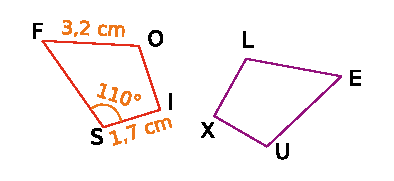
\includegraphics[width=5.9cm]{sans_axe} \end{center}
 \begin{enumerate}
 \item Reproduis et complète le tableau suivant.
 \begin{center}
  \begin{tabularx}{0.9\linewidth}{|c|*{6}{>{\centering\arraybackslash}X|}}
  \hline
\rowcolor{J1} Points & $F$ & $O$ & $I$ & $S$ \\ \hline
\rowcolor{C3} Symétriques & & & & \\ \hline
 \end{tabularx}
 \end{center}
 \vspace{0.3cm}
Tu justifieras ensuite chaque réponse.
 \item Quelle est la longueur du segment $[LE]$ ?
 \item Quelle autre longueur peux‑tu déterminer ?
 \item Quelle est la mesure de l'angle $\widehat{XUE}$ ?
 \item Écris deux autres égalités de mesure d'angles.
 \end{enumerate}
\end{exercice}


\begin{exercice}[À la recherche de l'axe]
Dans chaque cas, décalque les deux figures puis trace l'axe de symétrie. (Tu expliqueras comment tu fais sans plier le calque.)
 \begin{center} 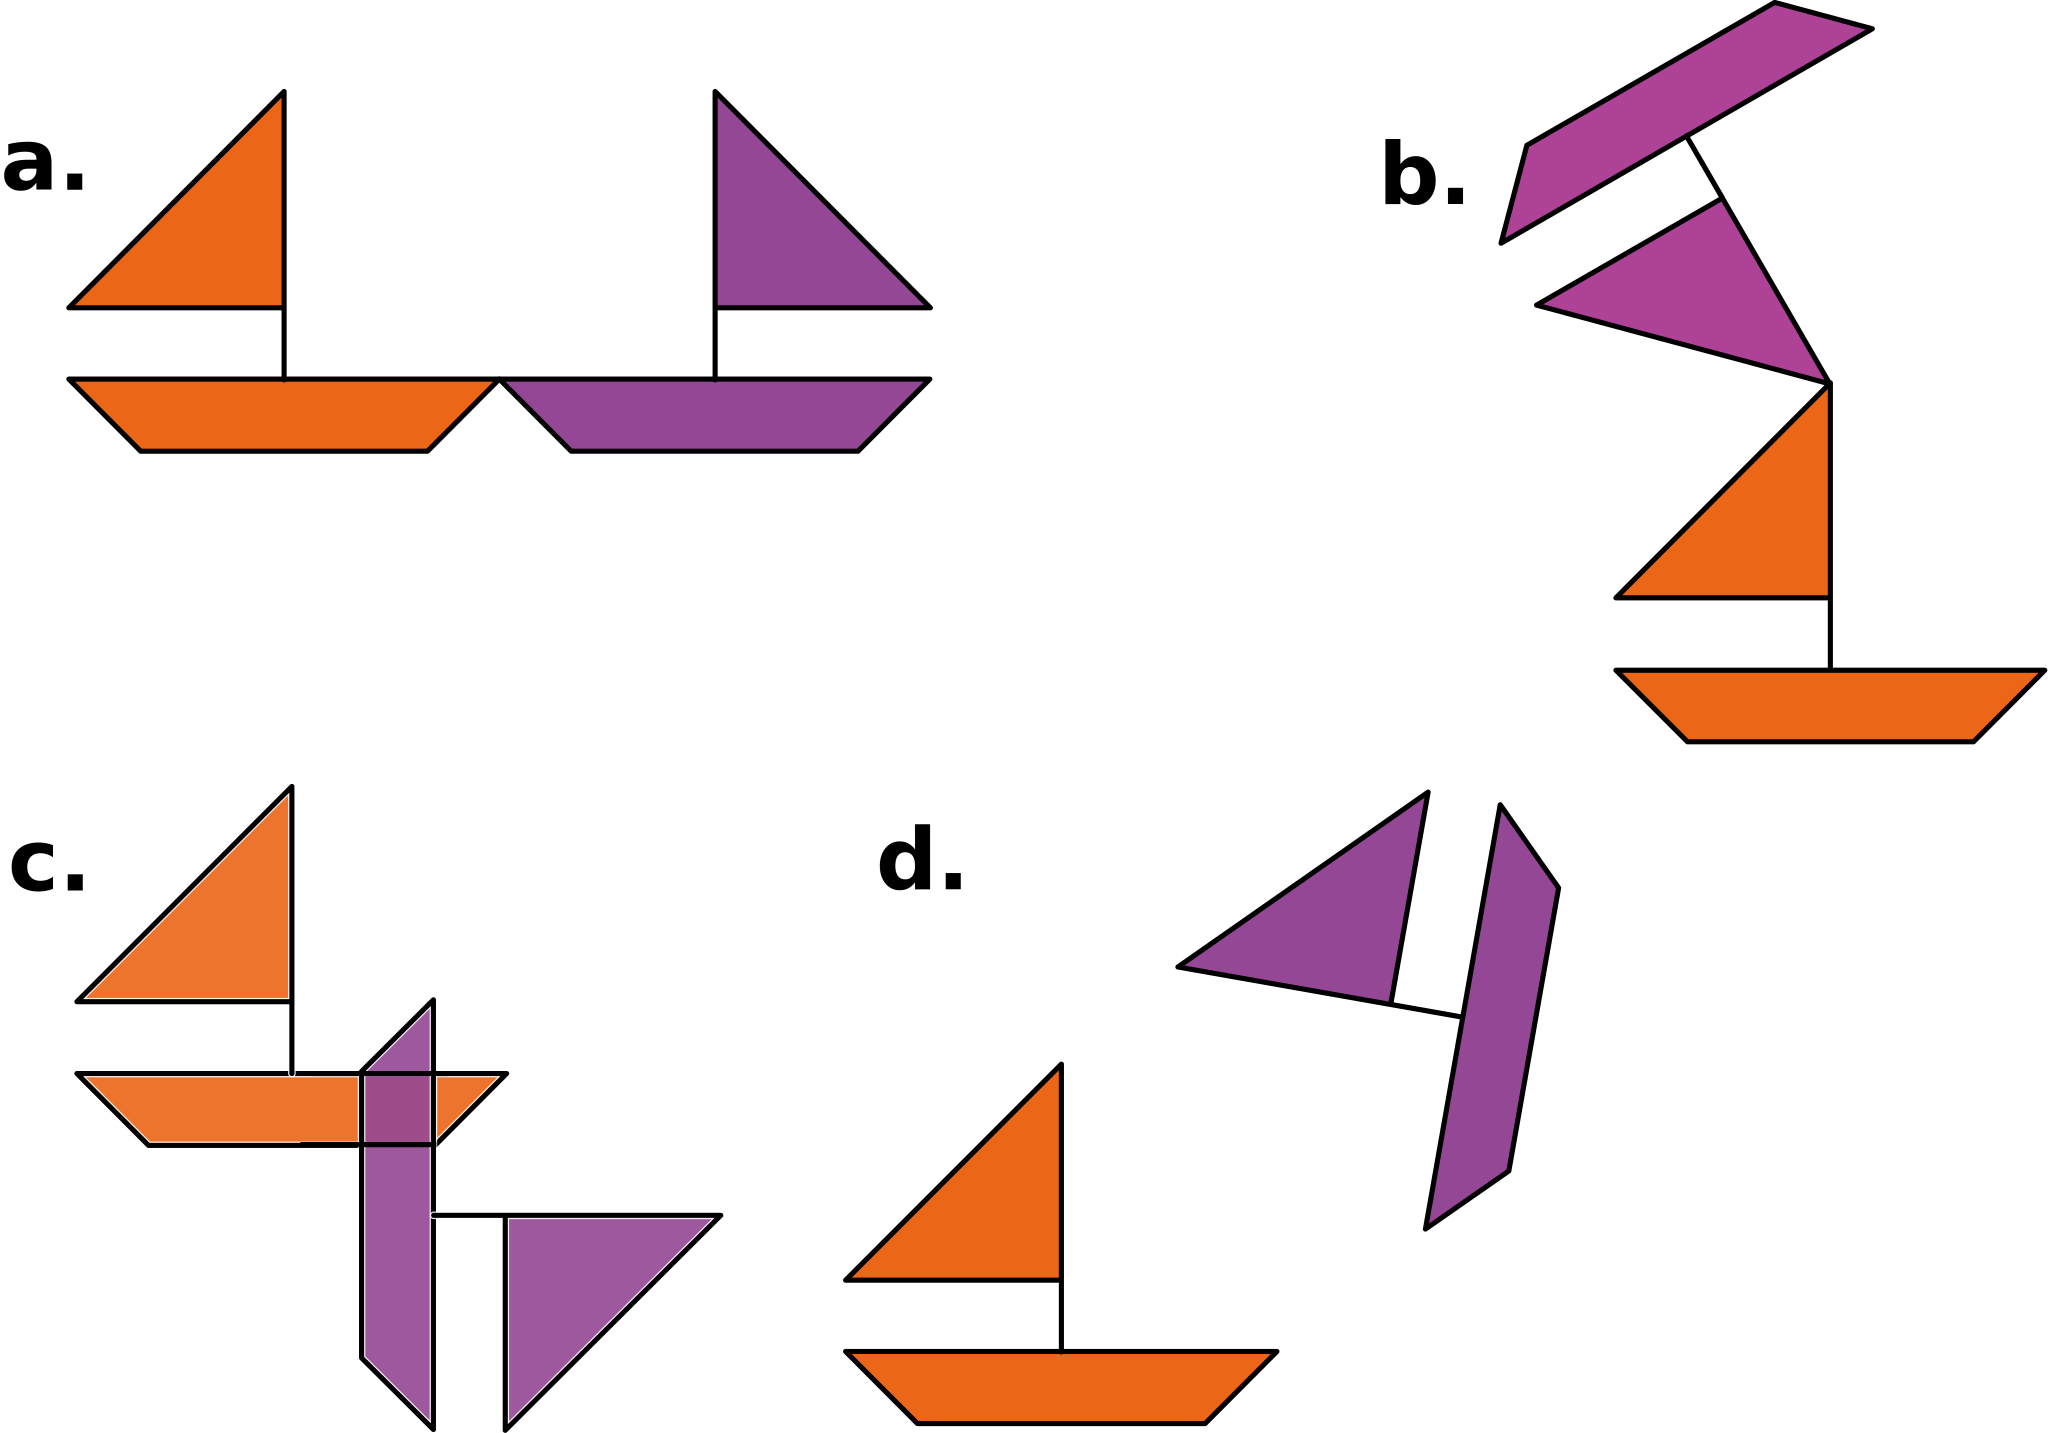
\includegraphics[width=8cm]{bateaux_colores} \end{center}
\end{exercice}

%%%%%%%%%%%%%%%%%%%%%%%%%%%%%%%%%%%%%%%%%%%%%%%%%%%%%%%%%%%%%%%%%%%%

\serie{Symétrie centrale}

\begin{exercice}
À l'aide de la règle graduée, retrouve, sur la figure ci-dessous, toutes les paires de points qui semblent symétriques par rapport au point $N$ : 
 \begin{center} 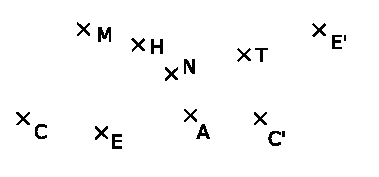
\includegraphics[width=5.8cm]{many_points} \end{center}
\end{exercice}


\begin{exercice}
Reforme des phrases correctes en associant les bonnes cases et recopie-les sur ton cahier :
\begin{center}
\renewcommand*\tabularxcolumn[1]{>{\centering\arraybackslash}m{#1}}
\begin{ttableau}{\linewidth}{3}
 \cline{1-1}\cline{3-3}
 \small{$A'$ est le symétrique du point $A$ par rapport au point $O$ donc \ldots} & & \small{$A'$ est le milieu du segment $[OA]$.} \\  \cline{1-1}\cline{3-3}
 \small{$O$ est l'image du point $A$ par la symétrie de centre $A'$ donc \ldots} & & \small{$A$ est le milieu du segment $[OA']$.} \\  \cline{1-1}\cline{3-3}
 \small{Le point $A'$ se transforme en $O$ par la symétrie de centre $A$ donc \ldots} & & \small{$O$ est le milieu du segment $[AA']$.} \\  \cline{1-1}\cline{3-3}
 \end{ttableau}
 \end{center}
\end{exercice}


\begin{exercice}
Dans chaque cas, reproduis la lettre sur du papier quadrillé et construis son symétrique par rapport au point $G$ :
 \begin{center} 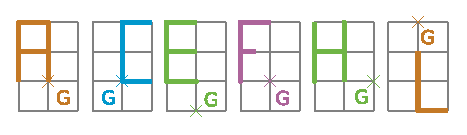
\includegraphics[width=7.7cm]{lettresG} \end{center}
\end{exercice}


\begin{exercice}
Sur ton cahier, reproduis la figure ci-dessous et construis les symétriques des points $P$, $R$ et $O$ par rapport au point $F$ :
 \begin{center} 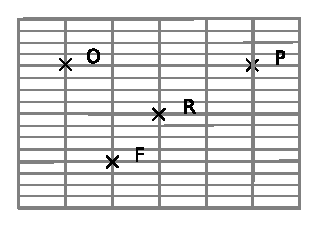
\includegraphics[width=5cm]{cahierFORP} \end{center}
\end{exercice}


\begin{exercice}
Sur ton cahier, reproduis la figure et construis le symétrique du mot MAT par rapport au point $R$ puis le symétrique du mot obtenu par rapport à la droite $d$ :
 \begin{center} \includegraphics[width=6.3cm]{MAT} \end{center}
\end{exercice}


\begin{exercice}
Dans chaque cas, reproduis la figure et construis le point $D$, symétrique du point $A$ par rapport au point $C$ puis le point $E$, symétrique du point $C$ par rapport au point $B$ :
\begin{colenumerate}{2}
 \item 
 
 \includegraphics[width=3.7cm]{symCAB1}
 \item 
 
 \includegraphics[width=3.7cm]{symCAB2}
 \end{colenumerate}
\end{exercice}


\begin{exercice}

\begin{minipage}[c]{0.48\linewidth}
Reproduis séparément chaque triangle sur du papier quadrillé et construis son symétrique par rapport au point $S$ :
 \end{minipage} \hfill%
 \begin{minipage}[c]{0.48\linewidth}
 \includegraphics[width=3.7cm]{triangles_symS}
 \end{minipage} \\
\end{exercice}


\begin{exercice}
Reproduis les figures ci-dessous sur du papier quadrillé et construis le symétrique de chacune d'elles par rapport au point $H$ :
\begin{colenumerate}{2}
 \item 

 \includegraphics[width=3.7cm]{maison_sym}

 \item
 
 \includegraphics[width=3.7cm]{champignon_sym}
 \end{colenumerate}
\end{exercice}


\begin{exercice}

\begin{minipage}[c]{0.48\linewidth}
Sur la figure ci-contre, $ROSE$ est un carré de centre $H$. Les points $I$, $J$, $K$ et $L$ sont les milieux respectifs des côtés $[RO]$, $[OS]$, $[SE]$ et $[RE]$.
 \end{minipage} \hfill%
\begin{minipage}[c]{0.48\linewidth}
 \includegraphics[width=3.7cm]{ROSE}
 \end{minipage} \\
 \begin{enumerate}
  \item Reproduis la figure en prenant $RO = 8$ cm ;
  \item Colorie en jaune le triangle $RNI$ ;
  \item Colorie en rouge le symétrique du triangle $RNI$ par rapport à la droite $(IK)$ puis en orange le symétrique du triangle $RNI$ par rapport à la droite $(LJ)$ ;
  \item Colorie en bleu le symétrique du triangle $RNI$ par rapport au point $N$ puis en vert le symétrique du triangle $RNI$ par rapport au point $H$.
 \end{enumerate}
\end{exercice}


\begin{exercice}
Dans chaque cas, des élèves ont voulu tracer la figure symétrique du bateau bleu par rapport au point $C$. Les tracés sont-ils exacts ? Explique pourquoi. 
\begin{colenumerate}{2}
 \item 
 
 \includegraphics[width=2.3cm]{bateaux_bn1}
 \item 
 
 \includegraphics[width=3.7cm]{bateaux_bn2}
 \item 
 
 \includegraphics[width=3.7cm]{bateaux_bn3}
 \item 
 
 \includegraphics[width=3.7cm]{bateaux_bn4}
 \end{colenumerate}
\end{exercice}


\begin{exercice}
Place trois points $A$, $B$ et $C$ non alignés tels que $AB = 5$ cm et $AC = 3$ cm. Construis, avec seulement la règle graduée, les points $B'$ et $C'$ symétriques respectifs des points $B$ et $C$ par rapport au point $A$.
\end{exercice}


\begin{exercice}
Reproduis la figure ci-dessous et construis, avec la règle non graduée et le compas, les symétriques des points $M$ et $R$ par rapport au point $E$ :
 \begin{center} \includegraphics[width=4.4cm]{pointsMER} \end{center}
\end{exercice}


\begin{exercice}
Reproduis chaque figure et construis le symétrique du segment $[AB]$ par rapport au point $S$ :
\begin{colenumerate}{3}
 \item 
 
 \includegraphics[width=2cm]{pointsSAB_1}
  \item 
 
 \includegraphics[width=2cm]{pointsSAB_2}
  \item 
 
 \includegraphics[width=2.5cm]{pointsSAB_3}
 \end{colenumerate}
\end{exercice}


\begin{exercice}
Reproduis chaque figure et construis le symétrique de la droite $d$ par rapport au point $U$ :
\begin{colenumerate}{2}
 \item 
 
 \includegraphics[width=3.5cm]{pointsUd}
  \item 
 
 \includegraphics[width=3.5cm]{pointsUd2}
 \end{colenumerate}
\end{exercice}


\begin{exercice}
Reproduis chaque figure en prenant 5 cm pour le rayon du cercle puis construis le symétrique du cercle par rapport au point $T$ :
\begin{colenumerate}{3}
 \item \includegraphics[width=2cm]{cercleKT1}
 \item \includegraphics[width=2cm]{cercleKT2}
 \item \includegraphics[width=1.4cm]{cercleKT3}
 \end{colenumerate}
\end{exercice}


\begin{exercice}
Construis un triangle $EFG$ rectangle en $E$ tel que $EF = 3$ cm et $EG = 5$ cm.
\begin{enumerate}
 \item Place le point $M$ milieu du segment $[EF]$ puis construis les points $E_1$, $F_1$ et $G_1$ symétriques respectifs des points $E$, $F$ et $G$ par rapport au point $M$ ;
 \item Construis les points $E_2$, $F_2$ et $G_2$ images respectives des points $E_1$, $F_1$ et $G_1$  par la symétrie de centre $E$ ;
 \item Place le point $K$ milieu du segment $[FG]$ puis construis les points $E_3$, $F_3$ et $G_3$ symétriques respectifs des points $E$, $F$ et $G$ par rapport au point $K$ ;
 \item Les points $E_3$, $F_3$ et $G_3$ sont les images respectives des points $E_2$, $F_2$ et $G_2$ par la symétrie de centre $O$. Quelle semble être la position de ce point $O$ ? Place-le sur ta figure.
 \end{enumerate}
\end{exercice}


\begin{exercice}[Figures complexes]
\begin{enumerate}
 \item Reproduis la figure ci-dessous, en haut à gauche avec $AB = 8$ cm et $AD = 5$ cm. Le point $E$ est le milieu du segment $[AB]$. 
 \begin{center} \includegraphics[width=5.2cm]{fig_complexes} \end{center}
 \item Construis le symétrique de cette figure par rapport au point $B$.
 \end{enumerate}
\end{exercice}


\begin{exercice}
Construis un rectangle $MATH$ tel que $MA = 5$ cm et $AT = 7$ cm puis place le point $E$ sur le côté $[AT]$ tel que $AE = 2$ cm. Construis en rouge le symétrique du rectangle $MATH$ par rapport au point $E$.
\end{exercice}


\begin{exercice}
Parmi les cartes ci-dessous, quelles sont celles qui possèdent un centre de symétrie ? 
 \begin{center} \includegraphics[width=7.7cm]{cartes_poker1} \end{center}
\end{exercice}


\begin{exercice}
Marine affirme que toutes les cartes ci-dessous possèdent un centre de symétrie. A-t-elle raison ? Justifie ta réponse.
 \begin{center} \includegraphics[width=7.7cm]{cartes_poker2} \end{center}
\end{exercice}


\begin{exercice}
Reproduis les lettres ci-dessous puis, trace en vert l'axe (ou les axes) de symétrie et en rouge le centre de symétrie de chaque lettre lorsqu'il(s) existe(nt) :
 \begin{center} \includegraphics[width=7.4cm]{lettres_grandes} \end{center}
\end{exercice}


\begin{exercice}
Sur la figure ci-dessous, le point $B$ est le symétrique du point $A$ par rapport à $O$ :
 \begin{center} \includegraphics[width=7.9cm]{quadrillageABCDE} \end{center}
\begin{enumerate}
 \item Reproduis la figure ci-dessus puis place le point $O$ ;
 \item En t'aidant du quadrillage, place les points $C'$, $D'$ et $E'$ symétriques respectifs des points $C$, $D$ et $E$ par rapport à $O$.
 \end{enumerate}
\end{exercice}


\begin{exercice}
Reproduis puis complète la figure ci-dessous pour que $O$ soit un centre de symétrie de celle-ci :
 \begin{center} \includegraphics[width=6.9cm]{quadrillage_figsym} \end{center}
\end{exercice}


\begin{exercice}
Reproduis puis colorie le minimum de cases pour que chacune des figures ci-dessous admette le point $O$ pour centre de symétrie :

\begin{minipage}[c]{0.48\linewidth}
\includegraphics[width=3.7cm]{carreaux_colores1}
 \end{minipage} \hfill%
\begin{minipage}[c]{0.48\linewidth}
 \includegraphics[width=3.7cm]{carreaux_colores2}
 \end{minipage} \\

\end{exercice}


\begin{exercice}
Reproduis la figure ci-dessous et complète-la de telle sorte que le centre du rectangle vert soit le centre de symétrie de la figure :
 \begin{center} \includegraphics[width=7.9cm]{fig_completer} \end{center}
\end{exercice}


\begin{exercice}[Nombres et centre de symétrie]
Christian a écrit les chiffres comme ci-dessous :
 \begin{center} \includegraphics[width=7.7cm]{nombres_grands} \end{center}
 \begin{enumerate}
  \item Il dit : « Si je fais le double du produit de 17 par 29, j'obtiens le plus grand nombre de trois chiffres différents qui possède un centre de symétrie. ». A-t-il raison ? 
  \item Trouve le plus petit nombre de trois chiffres différents dont l'écriture possède un centre de symétrie. Écris ce nombre et place le centre de symétrie.
  \end{enumerate}
\end{exercice}


\begin{exercice}
Soit un angle $\widehat{BAD}$ mesurant $120^\circ$ tel que $AB = 4$ cm et $AD = 5$ cm. Soit $C$ un point tel que le quadrilatère non croisé formé par les points $A$, $B$, $C$ et $D$ admette un centre de symétrie.
\begin{enumerate}
 \item Trace une figure à main levée.
 \item Combien y a-t-il de positions possibles pour le point $C$ ? Pour chaque cas, indique la position du centre de symétrie.
 \item Trace autant de figures qu'il y a de centres de symétrie et indique pour chaque cas le nom et la nature du quadrilatère ainsi construit.
 \end{enumerate}
\end{exercice}


\begin{exercice}
Éric a commencé la phrase suivante :
 \begin{center} « Le symétrique par rapport à $O$ d'un triangle isocèle est ... . ». \end{center}
 \begin{enumerate}
  \item Peux-tu compléter sa phrase ?
  \item Éric a oublié de justifier sa phrase. Fais-le pour lui.
  \item Écris deux autres phrases du même type en n'oubliant pas de justifier.
  \end{enumerate}
\end{exercice}


\begin{exercice}
On a tracé, à main levée, deux figures symétriques par rapport à $O$ :
 \begin{center} \includegraphics[width=7.9cm]{polygones_sym} \end{center}
\begin{enumerate}       
 \item Indique le symétrique par rapport à $O$ de chaque sommet du polygone $ABCDE$.
 \item Donne la longueur du segment $[PK]$. Justifie ta réponse.
 \item Donne la mesure de l'angle $\widehat{NPK}$. Justifie ta réponse.
 \item De quelles autres informations disposes-tu  concernant le polygone $KLMNP$ ? Pourquoi ?
 \end{enumerate}
\end{exercice}


\begin{exercice}[Histoire d'angles]
\begin{enumerate}
 \item Construis un angle $\widehat{xOy}$ mesurant $74^\circ$ puis place un point $A$ sur $[Ox)$ et un point $B$ sur $[Oy)$ ;
 \item Construis les points $C$ et $D$ symétriques respectifs de $B$ et de $O$ par rapport à $A$ ;
 \item Sans utiliser le rapporteur, mais en justifiant les réponses, donne la mesure de l'angle $\widehat{CDA}$ et compare les mesures des angles $\widehat{BAO}$ et $\widehat{DAC}$ ;
 \item Que peut-on dire des droites $(BD)$ et $(CO)$ ? Justifie ta réponse.
 \end{enumerate}
\end{exercice}


\begin{exercice}[Symétrie et périmètre]
\begin{enumerate}
 \item Trace un triangle $ABC$, isocèle en $A$ tel que $AB = 6$ cm et $BC = 3$ cm. Place le point $I$, milieu du segment $[BC]$ ;
 \item Construis le point $D$ symétrique du point $A$ par rapport à $I$ ;
 \item Donne les longueurs $DB$ et $DC$ puis le périmètre de $ABDC$ ;
 \item Quelle est la nature du quadrilatère $ABDC$ ? Justifie ta réponse.
 \end{enumerate}
\end{exercice}


\begin{exercice}
$ABC$ est un triangle tel que $AB = 4$ cm, $AC = 5$ cm et $BC = 6$ cm. $I$ désigne le milieu de $[AB]$ et $D$ le symétrique de $C$ par rapport à $I$.
\begin{enumerate}
 \item Construis la figure.
 \item Sans mesurer, mais en justifiant tes réponses, donne les mesures AD et BD.
 \end{enumerate}
\end{exercice}
\end{colonne*exercice}


\exercicesappr
\begin{colonne*exercice}

\begin{exercice}[Coloriage]
Reproduis et colorie le minimum de cases pour que la figure obtenue soit symétrique par rapport aux deux axes rouges :
\begin{center} \includegraphics[width=4.2cm]{coloriage_carre} \end{center}
\end{exercice}


\begin{exercice}[Une nouvelle construction]
\begin{enumerate}
 \item Trace à main levée une droite $d$ puis place deux points $M$ et $N$ sur $d$ et un point $B$ n'appartenant pas à $d$ ;
 \item Place, toujours à main levée, le point $B'$ symétrique de $B$ par rapport à $d$ ;
 \item Que peux‑tu dire de $MB$ et $MB'$ ? Justifie ta réponse et code la figure ;
 \item Que peux‑tu dire de $NB$ et $NB'$ ? Justifie ta réponse et code la figure ;
 \item Déduis‑en une méthode de construction du point $B'$ avec tes instruments de géométrie ;
 \item Trace la figure avec tes instruments de géométrie.
 \end{enumerate}
\end{exercice}


\begin{exercice}[L'axe invisible]
\begin{center} \includegraphics[width=7.2cm]{axe_invisible} \end{center}
Reproduis la figure ci‑dessus. Les points $C'$ et $D'$ sont les symétriques respectifs des points $C$ et $D$ par rapport à un axe invisible. \\[0.5em]
Construis les symétriques du cercle orange et du quadrilatère bleu par rapport à cet axe invisible.
\end{exercice}


\begin{exercice}[Mandala]
\begin{enumerate}
 \item Dessine un cercle de rayon 6 cm et deux de ses diamètres perpendiculaires. Tu obtiens quatre points sur le cercle. Trace tous les axes de symétrie de cette nouvelle figure. Tu obtiens de nouveaux points sur le cercle.
 \item Quel polygone obtiens‑tu en reliant tous ces points ? Combien a‑t‑il d'axes de symétrie ? Trace‑les tous.
 \item Poursuis en traçant un cercle de rayon 3 cm de même centre que celui de 6 cm. Reproduis le motif comme indiqué sur la figure 1 puis termine la construction et le coloriage en faisant des symétries successives par rapport aux axes (voir figure 2).
 \end{enumerate}
 \begin{minipage}[c]{0.48\linewidth}
 \includegraphics[width=4cm]{mandala1}
 \end{minipage} \hfill%
 \begin{minipage}[c]{0.48\linewidth}
 \includegraphics[width=4cm]{mandala2} 
  \end{minipage} \\
\begin{minipage}[c]{0.48\linewidth}
\begin{center} figure 1 \end{center}
 \end{minipage} \hfill%
 \begin{minipage}[c]{0.48\linewidth}
\begin{center} figure 2 \end{center}
  \end{minipage} \\
\end{exercice}


\begin{exercice}[Sans figure]
Melinda a réalisé une superbe figure et son symétrique. Malheureusement, elle a perdu sa feuille, mais sur son cahier, elle avait pris la précaution de faire le tableau suivant :
\begin{center}
\begin{tabularx}{0.9\linewidth}{|c|X|X|X|X|X|X|}
\hline
Points & E & T & R & S & A & C \\ \hline
Symétriques & V & J & I & S & Z & D\\ \hline
 \end{tabularx}
 \end{center}
Frédérique lui fait remarquer qu'avec un tel tableau, on peut obtenir des indications sans avoir besoin de la figure.
\begin{enumerate}
 \item Quel est le centre de la symétrie ?
 \item On sait que $ET = 3,4$ cm et $ZD = 5,1$ cm. Donne les longueurs $AC$ et $VJ$. Justifie.
 \item $RSA$ est un triangle équilatéral de 3 cm de côté. Quel autre triangle équilatéral est-on certain d'avoir sur la figure ? Justifie.
 \item On sait que $VJ = JI$. Quelle est la nature du triangle $ETR$ ? Pourquoi ?
 \end{enumerate}
\end{exercice}


\begin{exercice}[Symétrie et repère]
\begin{enumerate}
 \item Dessine un repère d'origine $O$ ayant pour unité le centimètre.
 \item Place les points : $I (1 ; 0)$ ; $A (2 ; 3)$ ; $B (6 ; - 1)$ ; $C (7 ; 3)$ ; $D (- 1 ; 1)$ ; $E (3 ; 0)$.
 \item Construis les points $F$, $G$, $H$ et $K$, symétriques respectifs de $A$, $B$, $C$ et $D$ par rapport à $O$.
 \item Donne les coordonnées de $F$, $G$, $H$ et $K$. Que remarques-tu ? \label{SymAxCent_approf}
 \item Donne les coordonnées des symétriques par rapport à $O$ des points $T (4 ; - 5)$ et $U (5 ; 0)$ sans les placer dans le repère.
 \item Place les points $M$, $N$, $P$ et $R$, symétriques respectifs des points $A$, $B$, $C$ et $D$ par rapport à $E$.
 \item Donne les coordonnées de $M$, $N$, $P$ et $R$. La propriété de la question \ref{SymAxCent_approf}. se vérifie-t-elle ici ? À quelle condition fonctionne-t-elle ?
 \end{enumerate}
\end{exercice}


\begin{exercice}
Reproduis la figure ci-dessous :
\begin{center} \includegraphics[width=3cm]{croixAOBd} \end{center}
\begin{enumerate}
 \item Construis les points $E$ et $F$, symétriques respectifs de $A$ et $B$ par rapport à $O$.
 \item Que peut-on dire des droites $(AB)$ et $(EF)$ ? Justifie ta réponse.
 \item Démontre que les droites $d$ et $(EF)$ sont perpendiculaires.
 \end{enumerate}
\end{exercice}


\begin{exercice}[Médiatrice et symétrie]
\begin{enumerate}
 \item Trace trois droites $d_1$, $d_2$ et $d_3$, concourantes en un point $O$ puis place :
 \begin{itemize}
  \item Sur $d_1$, $A$ et $A'$ tels que $OA = OA' = 3$ cm ;
  \item Sur $d_2$, $B$ et $B'$ tels que $OB = OB' = 4$ cm ;
  \item Sur $d_3$, $C$ et $C'$ tels que $OC = OC' = 5$ cm.
  \end{itemize}
 \item Démontre que $(B'C')$ et $(BC)$ sont parallèles.
 \item Construis la médiatrice d du segment $[BC]$.
 \item Démontre que $d$ est perpendiculaire à $(B'C')$.
 \end{enumerate}
\end{exercice}


\begin{exercice}[Pentagone et hexagone]
\underline{PARTIE A}
\begin{enumerate}
 \item Sur un cercle de centre $O$ et de rayon 4 cm, place un point $A$ puis quatre autres points distincts : $B$, $C$, $D$ et $E$ dans cet ordre tels que les angles $\widehat{AOB}$, $\widehat{BOC}$, $\widehat{COD}$, $\widehat{DOE}$ et $\widehat{EOA}$ mesurent tous $72^\circ$. 
 \item Trace le pentagone $ABCDE$. Que penses-tu des longueurs des côtés de ce pentagone ? Ce pentagone est appelé un pentagone régulier. A-t-il un centre de symétrie ?
\underline{PARTIE B}
 \item Sur un autre cercle de centre $O$ et de rayon 4 cm, place six points distincts $A$, $B$, $C$, $D$, $E$ et $F$ dans cet ordre tels que les angles $\widehat{AOB}$, $\widehat{BOC}$, $\widehat{COD}$, $\widehat{DOE}$, $\widehat{EOF}$ et $\widehat{FOA}$ mesurent tous $60^\circ$.
 \item Trace l'hexagone $ABCDEF$. Que penses-tu des longueurs des côtés de cet hexagone ? Cet hexagone est appelé un hexagone régulier. A-t-il un centre de symétrie ?
 \item Trace les triangles $ACE$ et $BDF$. Colorie avec plusieurs couleurs la figure en respectant la symétrie.
 \end{enumerate}
\end{exercice}



\end{colonne*exercice}

\connaissances
\begin{acquis}
\begin{itemize}
\item BlaBla1
\item BlaBla2
\item BlaBla3
\item BlaBla4
\item BlaBla5
\item BlaBla6
\end{itemize}
\end{acquis}

\QCMautoevaluation{Pour chaque question, plusieurs réponses sont
  proposées.  Déterminer celles qui sont correctes.}

\begin{QCM}
  \begin{GroupeQCM}
    \begin{exercice}
      Sur quelle(s) figure(s) les points $A$ et $B$ sont‑ils symétriques par rapport à $d$ ?
      \begin{ChoixQCM}{4}
      \item 
      
      \includegraphics[width=1.8cm]{1_R1}
      \item 
      
      \includegraphics[width=1.8cm]{1_R2}
      \item 
      
      \includegraphics[width=1.8cm]{1_R3}
      \item 
      
      \includegraphics[width=1.8cm]{1_R4}
      \end{ChoixQCM}
\begin{corrige}
     \reponseQCM{a} % j'ai mis "a" partout
   \end{corrige}
    \end{exercice}
    
    
    \begin{exercice}
      \begin{center} \includegraphics[width=2.9cm]{Q2} \end{center}
      \begin{ChoixQCM}{4}
      \item $A$ et $K$ sont symétriques par rapport à $d$
      \item $C$ est le symétrique de $M$ par rapport à $d$
      \item $ABC$ et $KLM$ sont symétriques par rapport à $d$
      \item $KL = AB$
      \end{ChoixQCM}
\begin{corrige}
     \reponseQCM{a}
   \end{corrige}
    \end{exercice}
    
    
    \begin{exercice}
      Dans quel(s) cas les triangles sont-ils symétriques par rapport à un axe ?
      \begin{ChoixQCM}{4}
      \item 
      
      \includegraphics[width=2.1cm]{3_R1}
      \item 
      
      \includegraphics[width=2.1cm]{3_R2}
      \item 
      
      \includegraphics[width=2.1cm]{3_R3}
      \item 
      
      \includegraphics[width=2.1cm]{3_R4}
      \end{ChoixQCM}
\begin{corrige}
     \reponseQCM{a}
   \end{corrige}
    \end{exercice}
    
    
    \begin{exercice}
      \begin{center} \includegraphics[width=3.1cm]{Q4} \end{center}
      \begin{ChoixQCM}{4}
      \item Les cercles noir et rouge sont symétriques par rapport à $d$
      \item Le cercle rouge est son propre symétrique par rapport à $d$
      \item Les cercles vert et rouge sont symétriques par rapport à $d$
      \item Les cercles bleu et noir sont symétriques par rapport à $d$
      \end{ChoixQCM}
\begin{corrige}
     \reponseQCM{a}
   \end{corrige}
    \end{exercice}
    \end{GroupeQCM}
\end{QCM}
    
\begin{QCM}
  \begin{GroupeQCM}
      \begin{exercice}
      Sur quelle(s) figure(s) les points $A$ et $B$ sont‑ils symétriques par rapport à $O$ ?
      \begin{ChoixQCM}{4}
      \item 
      
      \includegraphics[width=2.7cm]{5_R1}
      \item 
      
      \includegraphics[width=2.7cm]{5_R2}
      \item 
      
      \includegraphics[width=2.7cm]{5_R3}
      \item 
      
      \includegraphics[width=2.7cm]{5_R4}
      \end{ChoixQCM}
\begin{corrige}
     \reponseQCM{a}
   \end{corrige}
    \end{exercice}
    
    
    \begin{exercice}
      Dans quel(s) cas les triangles sont-ils symétriques par rapport au centre $O$ ?
      \begin{ChoixQCM}{4}
      \item 
      
      \includegraphics[width=2.7cm]{6_R1}
      \item 
      
      \includegraphics[width=2.7cm]{6_R2}
      \item 
      
      \includegraphics[width=2.7cm]{6_R3}
      \item 
      
      \includegraphics[width=2.7cm]{6_R4}
      \end{ChoixQCM}
\begin{corrige}
     \reponseQCM{a}
   \end{corrige}
    \end{exercice}
    \end{GroupeQCM}
\end{QCM}




  

\TravauxPratiques % pour nous "travailler en groupe"

\begin{TP}[Plusieurs symétries de suite \ldots]

Que se passe‑t‑il lorsqu'on fait subir à une figure plusieurs symétries axiales, l'une à la suite de l'autre ? \\[0.5em]
Par exemple, on construit d'abord le symétrique d'une figure par rapport à un axe $d$. On obtient une nouvelle figure, et on construit le symétrique de cette nouvelle figure par rapport à une autre droite $d'$. \\[0.5em]
Pour répondre à cette question, répartissez votre groupe en deux sous‑groupes. Le premier travaillera avec papier, crayon et instruments de géométrie. L'autre utilisera un logiciel de géométrie dynamique comme TracenPoche. \\[0.5em]
L'objectif de ce travail est de pouvoir répondre plus précisément aux questions suivantes.
\begin{enumerate}
 \item Que se passe‑t‑il si $d$ et $d'$ sont parallèles ?
 \item Que se passe‑t‑il si $d$ et $d'$ sont sécantes et non perpendiculaires en un point $O$ ?
 \item Que se passe‑t‑il si $d$ et $d'$ sont perpendiculaires ?
 \end{enumerate}
\begin{center} \includegraphics[width=6.7cm]{TracenPoche} \end{center}
\end{TP}

%%%%%%%%%%%%%%%%%%%%%%%%%%%%%%%%%%%%%%%%%%%%%%%%%%%%%%%%%%%%%%%%%%%%%%

\begin{TP}[Pavage rectangulaire]

Un pavage est une méthode de remplissage d'un espace à l'aide d'un motif répétitif, sans trou ni débordement.

\partie{Un pavage imposé}
\begin{enumerate}
\begin{minipage}[c]{0.58\linewidth}
 \item À partir d'une feuille au format A4, effectuez deux pliages pour obtenir quatre rectangles de même taille comme sur le schéma ci-contre.
 \end{minipage} \hfill%
 \begin{minipage}[c]{0.38\linewidth}
 \includegraphics[width=3.7cm]{pavage1234}
  \end{minipage} \\
 \item Sur votre feuille, construisez dans le rectangle \circled{1}, la figure ci-dessous ($O$ est le centre de l'arc de cercle) : ($AD = DO$ et $BI = IC$)
 \begin{center} \includegraphics[width=8.2cm]{pavageABCD} \end{center}
 \item Construisez le symétrique par rapport à $I$ de la figure tracée dans le rectangle \circled{1}. Dans quelle partie de la feuille va-t-il se situer ?
 \item Construisez les symétriques par rapport à la droite $(DC)$ des figures des parties \circled{1} et \circled{2}.
 \end{enumerate}
Rassemblez toutes les feuilles du groupe que vous placerez les unes à côté des autres pour former un grand rectangle. C'est un pavage rectangulaire.

\partie{Un pavage libre}
À partir de nouvelles feuilles A4, tracez, dans le rectangle  \circled{1}, un motif géométrique composé de droites, segments ou cercles. Tous les élèves du groupe doivent avoir exactement le même motif. \\[0.5em]
De la même façon qu'auparavant construisez l'image, par la symétrie de centre $I$, de la figure tracée dans le rectangle \circled{1} puis l'image, par la symétrie d'axe $(DC)$, des figures tracées dans les rectangles \circled{1} et \circled{2}. \\[0.5em]
En regroupant les feuilles, on obtient ainsi un nouveau pavage rectangulaire.
\end{TP}



\pagebreak

\recreation
\begin{enigme}[Optimisation de trajectoire]

\begin{minipage}[c]{0.58\linewidth} 
Dans un jeu vidéo, tu dois diriger ton héros mais les déplacements sont très longs. Ta mission est de partir de la ville $V$, de passer remplir ta gourde à la rivière et ensuite de rejoindre l'entrée du donjon $D$. Trace le trajet le plus court pour effectuer ta mission. (Indication : la distance la plus courte entre deux points reste la ligne droite.)

Ci-contre : la carte qui t'est donnée.
 \end{minipage} \hfill%
 \begin{minipage}[c]{0.38\linewidth}
 \includegraphics[width=5.5cm]{trajectoire}
  \end{minipage} \\
\end{enigme} 



